\documentclass{article} % For LaTeX2e
\usepackage{nips15submit_e,times}
\usepackage{hyperref}
\usepackage{url}
\usepackage{graphicx}
\usepackage{amsmath}
%\documentstyle[nips14submit_09,times,art10]{article} % For LaTeX 2.09


\title{Weekly Report(January.25,2019-March.4,2019)}

\author{Rui Shaopu}

	

\maketitle

\begin{abstract}
During the winter holiday, I learned several optimization algorithms first, then I also learnt a lot about classifiers and finished assignment 1 of cs231n.
\end{abstract}

\section{Learnt and Did}

Mainly I learned about classifiers and optimization algorithms. And I finished assignment 1, which gives me a big challenge, since I'm not familiar with python.

\subsection{Optimization Algorithms}
\subsubsection{Gradient Descent}
Usually we use this way to find the maximum value or the minimum value. We shall make it when the function is convex function.

Main formula:
\begin{center}
${\displaystyle J(\theta) = \frac{1}{2m}\sum_{i=1}^{m}(y_i-h_\theta(x_i))^2}$ 
\end{center}
partial derivation:
\begin{center}
${\displaystyle \theta'_j=\theta_j+(y_j-h_\theta(x_i))x_j^i}$
\end{center}
To get the value we want, we need to update parameters in the oppsite direction of gradient.

\subsubsection{Logistic Regression}
It is usually used to dedal with two classification problems since its unique attributes.

Main formula:
\begin{center}
${\displaystyle Y_w=\frac{1}{1+e^{-W^TX}}}$
\end{center}
Log likelihood function:
\begin{center}
${\displaystyle L(W)=-\frac{1}{m}\log({\prod_{i=1}^{m}[Y_w(X_i)]^{y_i}[1-Y_w(X_i)]^{1-y_i}})}$
\end{center}
Iterative formula($\alpha$ is learning rate):
\begin{center}
${\displaystyle W_j=\frac{\alpha}{m}\sum_{i=1}^{m}(Y_w(xi)-y_i)x_{ij}}$
\end{center}

\subsubsection{Newton's method}
Newton's method drops faster than gradient descent. However, it works bad when dealing with hessian matrix. 

Main formula:
\begin{center}
${\displaystyle x_{n+1}=x_n-\frac{f'(x_n)}{f"(x_n)}}$
\end{center}

Hessian matrix:
\begin{center}
${\displaystyle x_{n+1}=x_n-\frac{J_f(x_n)}{H(x_n)}}$

%\end{center}

${\displaystyle J_f(x_n)=}
% $
%$$
\left[
\begin{matrix} 
	\frac{\partial y_1}{\partial x_1} & \cdots & \frac{\partial y_n}{\partial x_1}\\
	\vdots & \ddots & \vdots \\
	\frac{y_1}{x_n} & \cdots & \frac{y_n}{x_n} 
\end{matrix}\quad
\right]
$

${\displaystyle H(x_n)=}
% $
%$$
\left[
\begin{matrix}
\frac{\partial^2 f}{\partial x_1^2}   & \cdots & \frac{\partial^2 f}{\partial x_1 \partial x_n}      \\
\vdots & \ddots & \vdots \\
\frac{\partial^2 f}{\partial x_n \partial x_1}   & \cdots & \frac{\partial^2 f}{\partial x_n^2}
\end{matrix}
\right]
% $
$

\end{center}

\subsection{Classifiers}

\subsubsection{KNN}
KNN, K Nearest Neighbor, One of the most easiest classifiers.

\begin{figure}[h]
	\centering  %插入的图片居中表示
	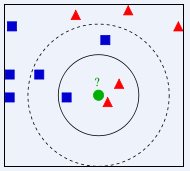
\includegraphics[width=.4\textwidth]{5.png} 
	\caption{2-dimension}  %图片的名称
	\label{fig:f5}   %标签,用作引用	
\end{figure}
In the training process of this algorithm, it stores all the input and output labels of training samples. in the test process, the distance between the test sample and each training sample L1 or L2 is calculated, then the first k training sample closest to test sample are selected. Then we'll vote on the label of the k samples, the category with the largest number of votes is categorized as test samples.

KNN is very easy, however it gets a bad result with classification accuracy of 27 percent. 

\subsubsection{SVM}
SVM, Support Vector Machine, is a kind of generalized linear classifier which classifies data by supervised learning. Its decision boundary is the maximum margin hyperplane for solving learning samples.

Under normal conditions, we use linear-SVM to classify two kinds of data, between which there is an obvious interval. However, if it doesn't exist, we need to find it in higher dimension. The figures below show it.

\begin{figure}[h]
	\centering  %插入的图片居中表示
	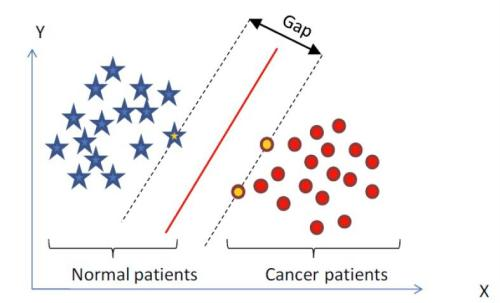
\includegraphics[width=.4\textwidth]{1.jpg} 
	\caption{2-dimension}  %图片的名称
	\label{fig:f1}   %标签,用作引用	
\end{figure}
\begin{figure}[h]
	\centering  %插入的图片居中表示
	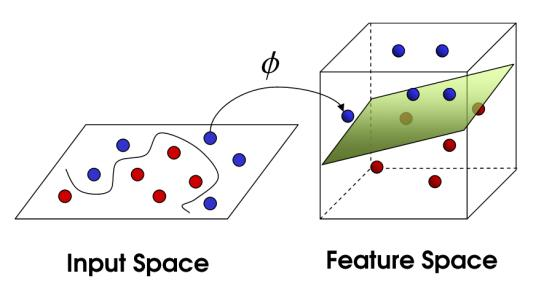
\includegraphics[width=.4\textwidth]{2.jpg}
	\caption{higher dimension}  %图片的名称
	\label{fig:f2}   %标签,用作引用
\end{figure}	

\subsubsection{Softmax}
In mathematics, the softmax function, also known as softargmax or normalized exponential function, is a function that takes as input a vector of K real numbers, and normalizes it into a probability distribution consisting of K probabilities. 

That is, after applying softmax, each component will be in the interval(0,1), and the components will add up to 1, so that they can be interpreted as probabilities. Furthermore, the larger input components will correspond to larger probabilities. Softmax is often used in neural networks and Often acts as an activation function of a neural network


The standard (unit) softmax function ${\displaystyle \sigma : {R} ^{K}\to {R} ^{K}}$ is defined by the formula

${\displaystyle \sigma (\mathbf {z} )_{j}={\frac {e^{z_{j}}}{\sum _{k=1}^{K}e^{z_{k}}}}}$
for j = 1, …, K and ${\displaystyle {\mathbf {z}}=(z_{1},\ldots ,z_{K})\in  {R} ^{K}}$


\subsubsection{Neural Network}
Neural network is a very important part of machine learning. As I know, Convolutional neural network is the most powerful one. In assignment 1, I need to finish a two-layer neural network. 

Main Formulas: 

Hyperplane: 
\begin{center}
	${\displaystyle y = W X+b}$
\end{center}

Activation function: 
\begin{center}
	${\displaystyle f_{sigmod} = \frac{1}{1+e^{z}}}$
\end{center}
Activation function derivation: 
\begin{center}
	${\displaystyle f'_{sigmod} = f_{sigmod}(1-f_{sigmod})}$
\end{center}

\begin{figure}[h]
	\centering  %插入的图片居中表示
	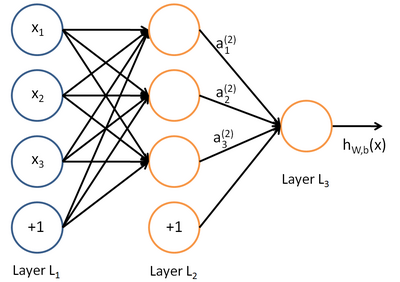
\includegraphics[width=.4\textwidth]{4.png} 
	\caption{2-dimension}  %图片的名称
	\label{fig:f3}
\end{figure}

\section{Problems}
The best problem I got is that I'm not familiar with Python libraries, such as numpy, matplotlib and so on. So was matrix operation. It took me a lot of time dealing with them and they still troubles me. My English is not very good too, I'm really gatefull that you finish reading it. Thanks a lot.

\section{Plan for Next Weeks}
In the following weeks, I will keep going and finish assignment 2. I will still learn to use python and latex familiarly.

\end{document}